\documentclass[11pt,a4paper]{article}
\usepackage[a4paper]{geometry}
\geometry{verbose,tmargin=2.5cm,bmargin=3.5cm,lmargin=2.54cm,rmargin=2.54cm}
\usepackage[T1]{fontenc}
\usepackage[mono=false]{libertine} \usepackage[libertine]{newtxmath}
\usepackage[english]{babel}
\usepackage[utf8]{inputenc}
\usepackage{longtable}
\usepackage{booktabs}

\usepackage{fancyhdr}
\pagestyle{fancy}
\lhead{\itshape $title$}
\chead{}
\rhead{\itshape{\nouppercase{\leftmark}}}
\lfoot{\itshape $for(author)$$author$$sep$ \\ $endfor$}
\cfoot{}
\rfoot{\itshape \thepage}

\usepackage{hyperref}
\hypersetup{
    colorlinks,
    citecolor=black,
    filecolor=black,
    linkcolor=black,
    urlcolor=black
}

\usepackage{graphicx}
\makeatletter
\def\maxwidth{\ifdim\Gin@nat@width>\linewidth\linewidth
\else\Gin@nat@width\fi}
\makeatother
\let\Oldincludegraphics\includegraphics
\renewcommand{\includegraphics}[1]{\Oldincludegraphics[width=\maxwidth]{#1}}




\begin{document}
\begin{titlepage}
\begin{center}
\vspace*{3.5 cm}

\textsc{\huge \bfseries $title$}\\[0.4cm]
%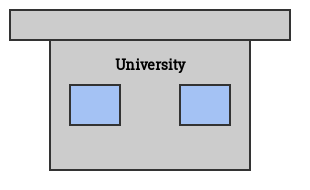
\includegraphics{unilogo.png}\\[0.5cm] %Uncomment to put a logo in the title
\textsc{\Large $for(author)$$author$$sep$ \\ $endfor$}\\[0.5cm]
\textsc{\Large \today}\\[0.5cm]


\end{center}
\end{titlepage}
\pagebreak

%$if(title)$
\maketitle
%$endif$

$if(toc)$
\tableofcontents
$if(tables)$
\listoftables
$endif$
$if(graphics)$
\listoffigures
$endif$
\pagebreak
$endif$

$body$

\end{document}
